% Options for packages loaded elsewhere
\PassOptionsToPackage{unicode}{hyperref}
\PassOptionsToPackage{hyphens}{url}
%
\documentclass[
]{article}
\usepackage{amsmath,amssymb}
\usepackage{lmodern}
\usepackage{ifxetex,ifluatex}
\ifnum 0\ifxetex 1\fi\ifluatex 1\fi=0 % if pdftex
  \usepackage[T1]{fontenc}
  \usepackage[utf8]{inputenc}
  \usepackage{textcomp} % provide euro and other symbols
\else % if luatex or xetex
  \usepackage{unicode-math}
  \defaultfontfeatures{Scale=MatchLowercase}
  \defaultfontfeatures[\rmfamily]{Ligatures=TeX,Scale=1}
\fi
% Use upquote if available, for straight quotes in verbatim environments
\IfFileExists{upquote.sty}{\usepackage{upquote}}{}
\IfFileExists{microtype.sty}{% use microtype if available
  \usepackage[]{microtype}
  \UseMicrotypeSet[protrusion]{basicmath} % disable protrusion for tt fonts
}{}
\makeatletter
\@ifundefined{KOMAClassName}{% if non-KOMA class
  \IfFileExists{parskip.sty}{%
    \usepackage{parskip}
  }{% else
    \setlength{\parindent}{0pt}
    \setlength{\parskip}{6pt plus 2pt minus 1pt}}
}{% if KOMA class
  \KOMAoptions{parskip=half}}
\makeatother
\usepackage{xcolor}
\IfFileExists{xurl.sty}{\usepackage{xurl}}{} % add URL line breaks if available
\IfFileExists{bookmark.sty}{\usepackage{bookmark}}{\usepackage{hyperref}}
\hypersetup{
  pdftitle={Homework 4},
  pdfauthor={Ethan Hoffman, Gabrielle Barsotti, and Halley McVeigh},
  hidelinks,
  pdfcreator={LaTeX via pandoc}}
\urlstyle{same} % disable monospaced font for URLs
\usepackage[margin=1in]{geometry}
\usepackage{color}
\usepackage{fancyvrb}
\newcommand{\VerbBar}{|}
\newcommand{\VERB}{\Verb[commandchars=\\\{\}]}
\DefineVerbatimEnvironment{Highlighting}{Verbatim}{commandchars=\\\{\}}
% Add ',fontsize=\small' for more characters per line
\usepackage{framed}
\definecolor{shadecolor}{RGB}{248,248,248}
\newenvironment{Shaded}{\begin{snugshade}}{\end{snugshade}}
\newcommand{\AlertTok}[1]{\textcolor[rgb]{0.94,0.16,0.16}{#1}}
\newcommand{\AnnotationTok}[1]{\textcolor[rgb]{0.56,0.35,0.01}{\textbf{\textit{#1}}}}
\newcommand{\AttributeTok}[1]{\textcolor[rgb]{0.77,0.63,0.00}{#1}}
\newcommand{\BaseNTok}[1]{\textcolor[rgb]{0.00,0.00,0.81}{#1}}
\newcommand{\BuiltInTok}[1]{#1}
\newcommand{\CharTok}[1]{\textcolor[rgb]{0.31,0.60,0.02}{#1}}
\newcommand{\CommentTok}[1]{\textcolor[rgb]{0.56,0.35,0.01}{\textit{#1}}}
\newcommand{\CommentVarTok}[1]{\textcolor[rgb]{0.56,0.35,0.01}{\textbf{\textit{#1}}}}
\newcommand{\ConstantTok}[1]{\textcolor[rgb]{0.00,0.00,0.00}{#1}}
\newcommand{\ControlFlowTok}[1]{\textcolor[rgb]{0.13,0.29,0.53}{\textbf{#1}}}
\newcommand{\DataTypeTok}[1]{\textcolor[rgb]{0.13,0.29,0.53}{#1}}
\newcommand{\DecValTok}[1]{\textcolor[rgb]{0.00,0.00,0.81}{#1}}
\newcommand{\DocumentationTok}[1]{\textcolor[rgb]{0.56,0.35,0.01}{\textbf{\textit{#1}}}}
\newcommand{\ErrorTok}[1]{\textcolor[rgb]{0.64,0.00,0.00}{\textbf{#1}}}
\newcommand{\ExtensionTok}[1]{#1}
\newcommand{\FloatTok}[1]{\textcolor[rgb]{0.00,0.00,0.81}{#1}}
\newcommand{\FunctionTok}[1]{\textcolor[rgb]{0.00,0.00,0.00}{#1}}
\newcommand{\ImportTok}[1]{#1}
\newcommand{\InformationTok}[1]{\textcolor[rgb]{0.56,0.35,0.01}{\textbf{\textit{#1}}}}
\newcommand{\KeywordTok}[1]{\textcolor[rgb]{0.13,0.29,0.53}{\textbf{#1}}}
\newcommand{\NormalTok}[1]{#1}
\newcommand{\OperatorTok}[1]{\textcolor[rgb]{0.81,0.36,0.00}{\textbf{#1}}}
\newcommand{\OtherTok}[1]{\textcolor[rgb]{0.56,0.35,0.01}{#1}}
\newcommand{\PreprocessorTok}[1]{\textcolor[rgb]{0.56,0.35,0.01}{\textit{#1}}}
\newcommand{\RegionMarkerTok}[1]{#1}
\newcommand{\SpecialCharTok}[1]{\textcolor[rgb]{0.00,0.00,0.00}{#1}}
\newcommand{\SpecialStringTok}[1]{\textcolor[rgb]{0.31,0.60,0.02}{#1}}
\newcommand{\StringTok}[1]{\textcolor[rgb]{0.31,0.60,0.02}{#1}}
\newcommand{\VariableTok}[1]{\textcolor[rgb]{0.00,0.00,0.00}{#1}}
\newcommand{\VerbatimStringTok}[1]{\textcolor[rgb]{0.31,0.60,0.02}{#1}}
\newcommand{\WarningTok}[1]{\textcolor[rgb]{0.56,0.35,0.01}{\textbf{\textit{#1}}}}
\usepackage{graphicx}
\makeatletter
\def\maxwidth{\ifdim\Gin@nat@width>\linewidth\linewidth\else\Gin@nat@width\fi}
\def\maxheight{\ifdim\Gin@nat@height>\textheight\textheight\else\Gin@nat@height\fi}
\makeatother
% Scale images if necessary, so that they will not overflow the page
% margins by default, and it is still possible to overwrite the defaults
% using explicit options in \includegraphics[width, height, ...]{}
\setkeys{Gin}{width=\maxwidth,height=\maxheight,keepaspectratio}
% Set default figure placement to htbp
\makeatletter
\def\fps@figure{htbp}
\makeatother
\setlength{\emergencystretch}{3em} % prevent overfull lines
\providecommand{\tightlist}{%
  \setlength{\itemsep}{0pt}\setlength{\parskip}{0pt}}
\setcounter{secnumdepth}{-\maxdimen} % remove section numbering
\usepackage{booktabs}
\usepackage{longtable}
\usepackage{array}
\usepackage{multirow}
\usepackage{wrapfig}
\usepackage{float}
\usepackage{colortbl}
\usepackage{pdflscape}
\usepackage{tabu}
\usepackage{threeparttable}
\usepackage{threeparttablex}
\usepackage[normalem]{ulem}
\usepackage{makecell}
\usepackage{xcolor}
\ifluatex
  \usepackage{selnolig}  % disable illegal ligatures
\fi

\title{Homework 4}
\author{Ethan Hoffman, Gabrielle Barsotti, and Halley McVeigh}
\date{5/22/2021}

\begin{document}
\maketitle

\hypertarget{question-1}{%
\subsubsection{Question 1}\label{question-1}}

\begin{Shaded}
\begin{Highlighting}[]
\CommentTok{\#Question 1}
\DocumentationTok{\#\#Read in the damages.csv file and then mutate to set up the quadratic equation}
\NormalTok{damages }\OtherTok{\textless{}{-}} \FunctionTok{read.csv}\NormalTok{(}\FunctionTok{here}\NormalTok{(}\StringTok{"data"}\NormalTok{, }\StringTok{"damages.csv"}\NormalTok{)) }\SpecialCharTok{\%\textgreater{}\%} 
  \FunctionTok{mutate}\NormalTok{(}\AttributeTok{warm2 =}\NormalTok{ warming}\SpecialCharTok{\^{}}\DecValTok{2}\NormalTok{)}

\DocumentationTok{\#\#Create a linear model to find the estimated damage function in the damages data table}
\NormalTok{damages\_lm }\OtherTok{\textless{}{-}} \FunctionTok{lm}\NormalTok{(damages }\SpecialCharTok{\textasciitilde{}}\NormalTok{ warming }\SpecialCharTok{+}\NormalTok{ warm2, }\AttributeTok{data =}\NormalTok{ damages)}
\NormalTok{damages\_lm[[}\StringTok{"coefficients"}\NormalTok{]][[}\StringTok{"(Intercept)"}\NormalTok{]] }\OtherTok{\textless{}{-}} \DecValTok{0}

\DocumentationTok{\#\#Create data visualization of damages.csv data}
\FunctionTok{ggplot}\NormalTok{(}\AttributeTok{data =}\NormalTok{ damages, }\FunctionTok{aes}\NormalTok{ (}\AttributeTok{x =}\NormalTok{ warming, }\AttributeTok{y =}\NormalTok{ damages))}\SpecialCharTok{+}
  \FunctionTok{geom\_point}\NormalTok{() }\SpecialCharTok{+}
  \FunctionTok{geom\_smooth}\NormalTok{(}\AttributeTok{data=}\NormalTok{damages, }\FunctionTok{aes}\NormalTok{(}\AttributeTok{x=}\NormalTok{warming, }\AttributeTok{y=}\NormalTok{damages))}\SpecialCharTok{+}
  \FunctionTok{annotate}\NormalTok{(}\AttributeTok{geom =} \StringTok{"text"}\NormalTok{, }\AttributeTok{x =} \FloatTok{3.5}\NormalTok{, }\AttributeTok{y =} \DecValTok{1000000000000000}\NormalTok{, }\AttributeTok{label =} \StringTok{"y = 1.95 * (10\^{}{-}13) x\^{}2 {-} 3.07 * (10\^{}{-}12) x"}\NormalTok{) }\SpecialCharTok{+}
  \FunctionTok{theme\_minimal}\NormalTok{() }\SpecialCharTok{+}
  \FunctionTok{labs}\NormalTok{(}\AttributeTok{x =} \StringTok{"Warming (degrees C)"}\NormalTok{, }\AttributeTok{y =} \StringTok{"Damages ($)"}\NormalTok{, }\AttributeTok{title =} \StringTok{"Damages of climate change under different climate trajectories"}\NormalTok{)}
\end{Highlighting}
\end{Shaded}

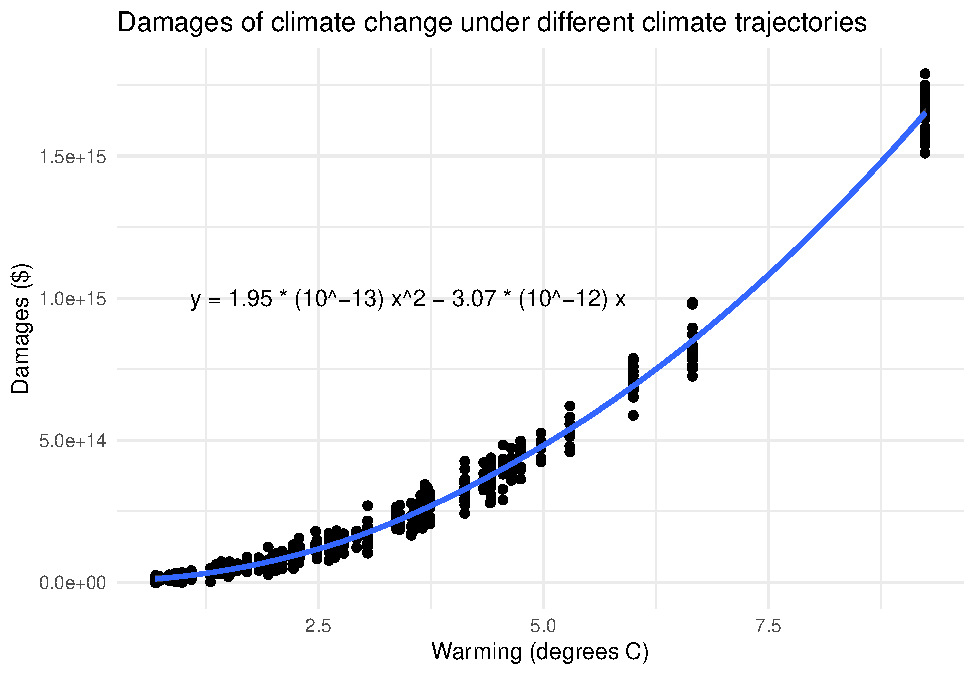
\includegraphics{Homework-4-Code_files/figure-latex/unnamed-chunk-1-1.pdf}

\hypertarget{question-2}{%
\subsubsection{Question 2}\label{question-2}}

\begin{Shaded}
\begin{Highlighting}[]
\CommentTok{\#Question 2}
\DocumentationTok{\#\#Read in the warming.csv file}
\NormalTok{warming }\OtherTok{\textless{}{-}} \FunctionTok{read.csv}\NormalTok{(}\FunctionTok{here}\NormalTok{(}\StringTok{"data"}\NormalTok{, }\StringTok{"warming.csv"}\NormalTok{))}
\end{Highlighting}
\end{Shaded}

\begin{Shaded}
\begin{Highlighting}[]
\CommentTok{\#Question 2}
\DocumentationTok{\#\#Use the warming file and estimated damage function from Question 1 to create four plots}
\DocumentationTok{\#\#\#Using the damages lm from Question 1, isolate the coefficient values to create this next graph.}
\NormalTok{x }\OtherTok{\textless{}{-}}\NormalTok{ damages\_lm[[}\StringTok{"coefficients"}\NormalTok{]][[}\StringTok{"warming"}\NormalTok{]]}
\NormalTok{x2 }\OtherTok{\textless{}{-}}\NormalTok{ damages\_lm[[}\StringTok{"coefficients"}\NormalTok{]][[}\StringTok{"warm2"}\NormalTok{]]}
\NormalTok{intercept }\OtherTok{\textless{}{-}}\NormalTok{ damages\_lm[[}\StringTok{"coefficients"}\NormalTok{]][[}\StringTok{"(Intercept)"}\NormalTok{]]}

\DocumentationTok{\#\#\#Find the Difference in Damages over Time that Arise from the Pulse. After finding the difference, divide the difference by 35 billion tons of carbon which is roughly equal to the amount of annual global emissions}
\NormalTok{warming\_difference }\OtherTok{\textless{}{-}}\NormalTok{ warming }\SpecialCharTok{\%\textgreater{}\%}
  \FunctionTok{mutate}\NormalTok{(}\AttributeTok{damage\_base =}\NormalTok{ (warming\_baseline}\SpecialCharTok{*}\NormalTok{x) }\SpecialCharTok{+}\NormalTok{ ((warming\_baseline)}\SpecialCharTok{\^{}}\DecValTok{2}\SpecialCharTok{*}\NormalTok{x2) }\SpecialCharTok{+}\NormalTok{ intercept,}
         \AttributeTok{damage\_high =}\NormalTok{ ((warming\_baseline}\SpecialCharTok{*}\FloatTok{1.5}\NormalTok{)}\SpecialCharTok{*}\NormalTok{x) }\SpecialCharTok{+}\NormalTok{ ((warming\_baseline}\SpecialCharTok{*}\FloatTok{1.5}\NormalTok{)}\SpecialCharTok{\^{}}\DecValTok{2}\SpecialCharTok{*}\NormalTok{x2) }\SpecialCharTok{+}\NormalTok{ intercept,}
         \AttributeTok{damage\_pulse =}\NormalTok{ (warming\_pulse }\SpecialCharTok{*}\NormalTok{ x) }\SpecialCharTok{+}\NormalTok{ ((warming\_pulse)}\SpecialCharTok{\^{}}\DecValTok{2} \SpecialCharTok{*}\NormalTok{ x2) }\SpecialCharTok{+}\NormalTok{ intercept,}
         \AttributeTok{damage\_difference =}\NormalTok{ damage\_pulse }\SpecialCharTok{{-}}\NormalTok{ damage\_base,}
         \AttributeTok{damage\_annual\_cost =}\NormalTok{ damage\_difference}\SpecialCharTok{/}\DecValTok{35000000000}
\NormalTok{         )}
\end{Highlighting}
\end{Shaded}

\hypertarget{plot-1-4}{%
\paragraph{Plot 1-4}\label{plot-1-4}}

\begin{Shaded}
\begin{Highlighting}[]
\DocumentationTok{\#\#\#Damages Over Time without the Pulse}
\NormalTok{damage\_plot }\OtherTok{\textless{}{-}} \FunctionTok{ggplot}\NormalTok{(}\AttributeTok{data =}\NormalTok{ warming\_difference, }\FunctionTok{aes}\NormalTok{(}\AttributeTok{x =}\NormalTok{ year, }\AttributeTok{y =}\NormalTok{ damage\_base))}\SpecialCharTok{+}
  \FunctionTok{geom\_point}\NormalTok{()}\SpecialCharTok{+}
  \FunctionTok{theme\_minimal}\NormalTok{() }\SpecialCharTok{+}
  \FunctionTok{labs}\NormalTok{(}\AttributeTok{title =} \StringTok{"Plot 1: Damages over time without pulse"}\NormalTok{, }\AttributeTok{x =} \StringTok{"Year"}\NormalTok{, }\AttributeTok{y =} \StringTok{"Damages ($)"}\NormalTok{)}

\NormalTok{damage\_plot}
\end{Highlighting}
\end{Shaded}

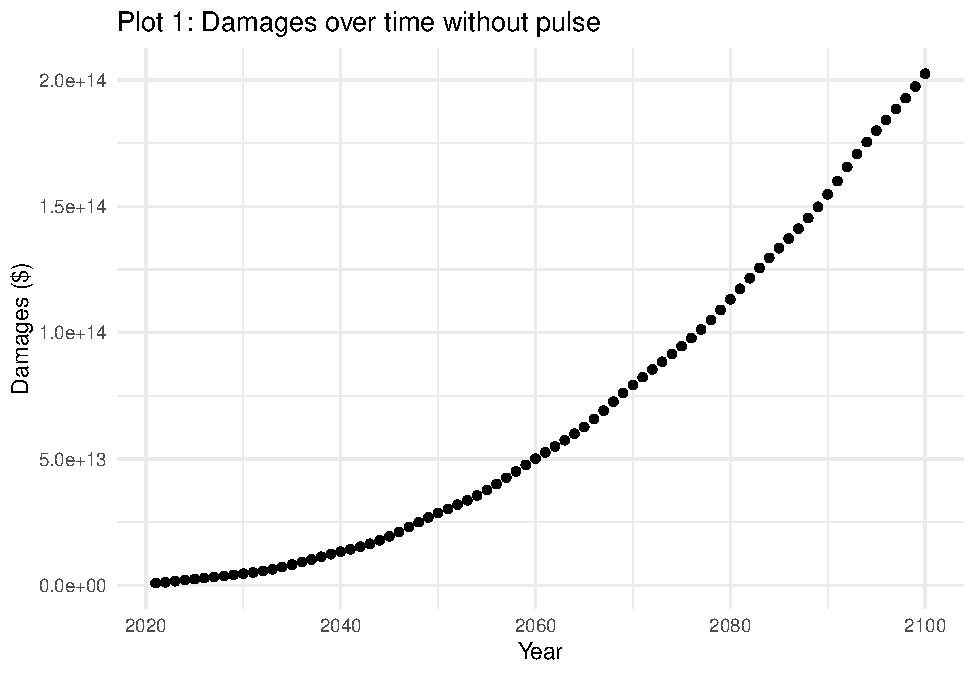
\includegraphics{Homework-4-Code_files/figure-latex/unnamed-chunk-4-1.pdf}

\begin{Shaded}
\begin{Highlighting}[]
\DocumentationTok{\#\#\#Damages Over Time with the Pulse}
\NormalTok{damage\_pulse\_plot }\OtherTok{\textless{}{-}} \FunctionTok{ggplot}\NormalTok{(}\AttributeTok{data =}\NormalTok{ warming\_difference, }\FunctionTok{aes}\NormalTok{(}\AttributeTok{x =}\NormalTok{ year, }\AttributeTok{y =}\NormalTok{ damage\_pulse))}\SpecialCharTok{+}
  \FunctionTok{geom\_point}\NormalTok{()}\SpecialCharTok{+}
  \FunctionTok{theme\_minimal}\NormalTok{() }\SpecialCharTok{+}
  \FunctionTok{labs}\NormalTok{(}\AttributeTok{title =} \StringTok{"Plot 2: Damages over time with pulse"}\NormalTok{, }\AttributeTok{x =} \StringTok{"Year"}\NormalTok{, }\AttributeTok{y =} \StringTok{"Damages ($)"}\NormalTok{)}

\NormalTok{damage\_pulse\_plot}
\end{Highlighting}
\end{Shaded}

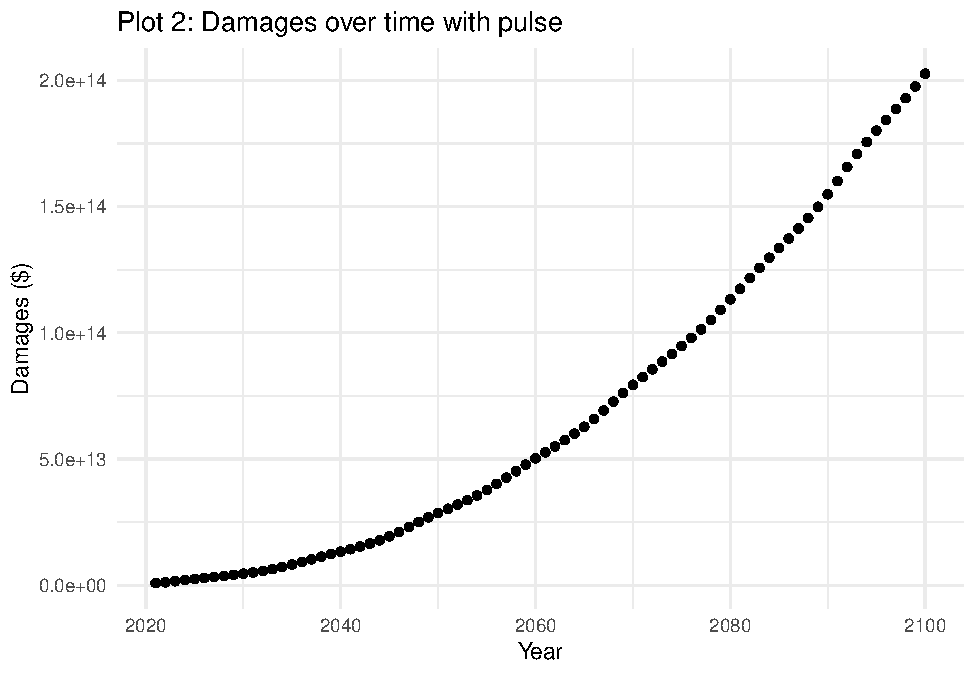
\includegraphics{Homework-4-Code_files/figure-latex/unnamed-chunk-4-2.pdf}

\begin{Shaded}
\begin{Highlighting}[]
\DocumentationTok{\#\#\#Damage difference Over Time without the Pulse}
\NormalTok{damage\_difference\_plot }\OtherTok{\textless{}{-}} \FunctionTok{ggplot}\NormalTok{(}\AttributeTok{data =}\NormalTok{ warming\_difference, }\FunctionTok{aes}\NormalTok{(}\AttributeTok{x =}\NormalTok{ year, }\AttributeTok{y =}\NormalTok{ damage\_difference))}\SpecialCharTok{+}
  \FunctionTok{geom\_point}\NormalTok{()}\SpecialCharTok{+}
  \FunctionTok{theme\_minimal}\NormalTok{() }\SpecialCharTok{+}
  \FunctionTok{labs}\NormalTok{(}\AttributeTok{title =} \StringTok{"Plot 3: Differences in damages over time from pulse"}\NormalTok{, }\AttributeTok{x =} \StringTok{"Year"}\NormalTok{, }\AttributeTok{y =} \StringTok{"Damages ($)"}\NormalTok{)}

\NormalTok{damage\_difference\_plot}
\end{Highlighting}
\end{Shaded}

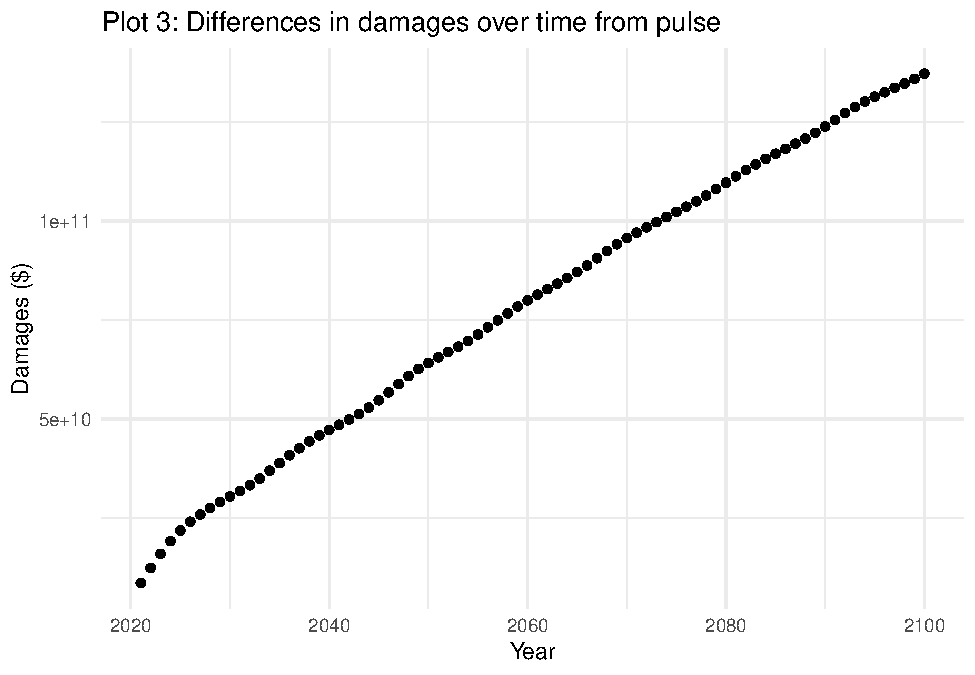
\includegraphics{Homework-4-Code_files/figure-latex/unnamed-chunk-4-3.pdf}

\begin{Shaded}
\begin{Highlighting}[]
\DocumentationTok{\#\#\#Damage difference over time per ton of carbon}
\NormalTok{damage\_ton\_plot }\OtherTok{\textless{}{-}} \FunctionTok{ggplot}\NormalTok{(}\AttributeTok{data =}\NormalTok{ warming\_difference, }\FunctionTok{aes}\NormalTok{(}\AttributeTok{x =}\NormalTok{ year, }\AttributeTok{y =}\NormalTok{ damage\_annual\_cost)) }\SpecialCharTok{+}
  \FunctionTok{geom\_point}\NormalTok{() }\SpecialCharTok{+}
  \FunctionTok{theme\_minimal}\NormalTok{() }\SpecialCharTok{+}
  \FunctionTok{labs}\NormalTok{(}\AttributeTok{title =} \StringTok{"Plot 4: Difference in damages over time from pulse per ton of CO2"}\NormalTok{, }\AttributeTok{x =} \StringTok{"Year"}\NormalTok{, }\AttributeTok{y =} \StringTok{"Damages ($)"}\NormalTok{)}

\NormalTok{damage\_ton\_plot}
\end{Highlighting}
\end{Shaded}

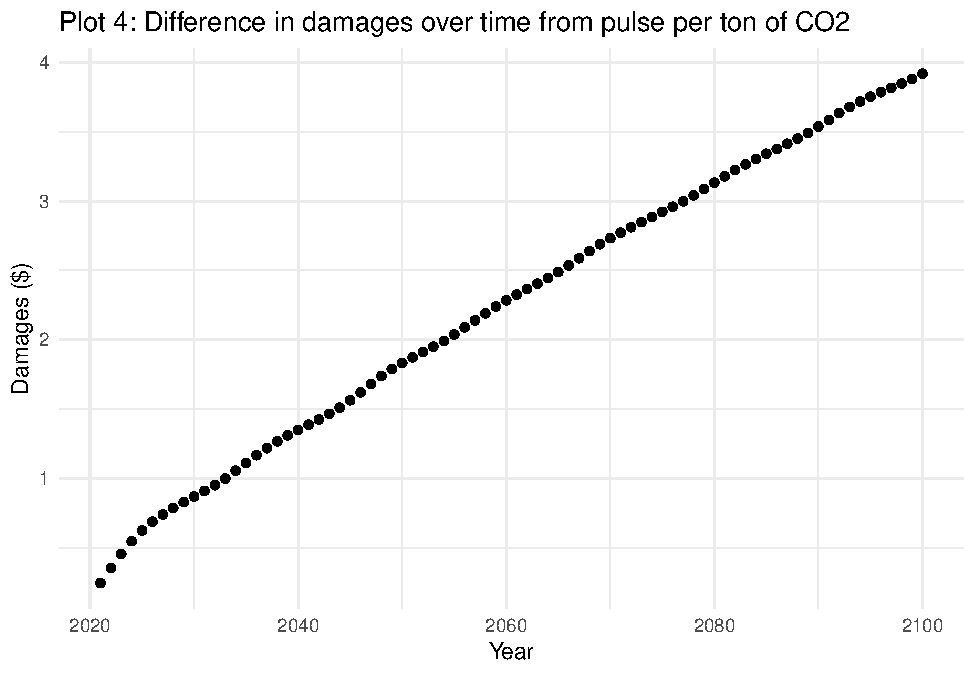
\includegraphics{Homework-4-Code_files/figure-latex/unnamed-chunk-4-4.pdf}

\hypertarget{question-3}{%
\subsubsection{Question 3}\label{question-3}}

\begin{Shaded}
\begin{Highlighting}[]
\CommentTok{\#Question 3}
\DocumentationTok{\#\#Create a plot of SCC vs. Discount Rate}
\NormalTok{warming\_scc }\OtherTok{\textless{}{-}}\NormalTok{ warming\_difference}

\NormalTok{warming\_scc }\OtherTok{\textless{}{-}}\NormalTok{ warming\_difference }\SpecialCharTok{\%\textgreater{}\%} 
  \FunctionTok{mutate}\NormalTok{(}\AttributeTok{Discount1 =}\NormalTok{ ((}\FunctionTok{sum}\NormalTok{(warming\_scc}\SpecialCharTok{$}\NormalTok{damage\_annual\_cost))}\SpecialCharTok{/}\NormalTok{(}\DecValTok{1}\FloatTok{+0.01}\NormalTok{)}\SpecialCharTok{\^{}}\DecValTok{80}\NormalTok{),}
         \AttributeTok{Discount2 =}\NormalTok{ ((}\FunctionTok{sum}\NormalTok{(warming\_scc}\SpecialCharTok{$}\NormalTok{damage\_annual\_cost))}\SpecialCharTok{/}\NormalTok{(}\DecValTok{1}\FloatTok{+0.02}\NormalTok{)}\SpecialCharTok{\^{}}\DecValTok{80}\NormalTok{),}
         \AttributeTok{Discount3 =}\NormalTok{ ((}\FunctionTok{sum}\NormalTok{(warming\_scc}\SpecialCharTok{$}\NormalTok{damage\_annual\_cost))}\SpecialCharTok{/}\NormalTok{(}\DecValTok{1}\FloatTok{+0.03}\NormalTok{)}\SpecialCharTok{\^{}}\DecValTok{80}\NormalTok{),}
         \AttributeTok{Discount4 =}\NormalTok{ ((}\FunctionTok{sum}\NormalTok{(warming\_scc}\SpecialCharTok{$}\NormalTok{damage\_annual\_cost))}\SpecialCharTok{/}\NormalTok{(}\DecValTok{1}\FloatTok{+0.04}\NormalTok{)}\SpecialCharTok{\^{}}\DecValTok{80}\NormalTok{),}
         \AttributeTok{Discount5 =}\NormalTok{ ((}\FunctionTok{sum}\NormalTok{(warming\_scc}\SpecialCharTok{$}\NormalTok{damage\_annual\_cost))}\SpecialCharTok{/}\NormalTok{(}\DecValTok{1}\FloatTok{+0.05}\NormalTok{)}\SpecialCharTok{\^{}}\DecValTok{80}\NormalTok{))}

\NormalTok{scc\_table }\OtherTok{\textless{}{-}}\NormalTok{ warming\_scc }\SpecialCharTok{\%\textgreater{}\%} 
  \FunctionTok{select}\NormalTok{(}\StringTok{"Discount1"}\NormalTok{, }\StringTok{"Discount2"}\NormalTok{, }\StringTok{"Discount3"}\NormalTok{, }\StringTok{"Discount4"}\NormalTok{, }\StringTok{"Discount5"}\NormalTok{) }\SpecialCharTok{\%\textgreater{}\%} 
  \FunctionTok{slice}\NormalTok{(}\DecValTok{1}\NormalTok{)}

\NormalTok{scc\_table}
\end{Highlighting}
\end{Shaded}

\begin{verbatim}
##   Discount1 Discount2 Discount3 Discount4 Discount5
## 1  81.23011  36.93288  16.92189  7.811956  3.633147
\end{verbatim}

\begin{Shaded}
\begin{Highlighting}[]
\NormalTok{trans\_scc\_table }\OtherTok{\textless{}{-}} \FunctionTok{t}\NormalTok{(scc\_table)}

\NormalTok{discount\_scc }\OtherTok{=} \FunctionTok{data.table}\NormalTok{(}
  \AttributeTok{SCC =} \FunctionTok{c}\NormalTok{(}\FloatTok{81.2301056376792}\NormalTok{, }\FloatTok{36.9328804024112}\NormalTok{, }\FloatTok{16.9218929850311}\NormalTok{, }\FloatTok{7.8119557882259}\NormalTok{, }\FloatTok{3.6331472085021}\NormalTok{),}
  \AttributeTok{Discount\_rate =} \FunctionTok{c}\NormalTok{(}\DecValTok{1}\NormalTok{, }\DecValTok{2}\NormalTok{, }\DecValTok{3}\NormalTok{, }\DecValTok{4}\NormalTok{, }\DecValTok{5}\NormalTok{)}
\NormalTok{)}

\NormalTok{discount\_scc}
\end{Highlighting}
\end{Shaded}

\begin{verbatim}
##          SCC Discount_rate
## 1: 81.230106             1
## 2: 36.932880             2
## 3: 16.921893             3
## 4:  7.811956             4
## 5:  3.633147             5
\end{verbatim}

\begin{Shaded}
\begin{Highlighting}[]
\FunctionTok{ggplot}\NormalTok{(}\AttributeTok{data =}\NormalTok{ discount\_scc, }\FunctionTok{aes}\NormalTok{(}\AttributeTok{x =}\NormalTok{ Discount\_rate, }\AttributeTok{y =}\NormalTok{ SCC)) }\SpecialCharTok{+}
  \FunctionTok{geom\_point}\NormalTok{() }\SpecialCharTok{+}
  \FunctionTok{geom\_smooth}\NormalTok{(}\AttributeTok{data =}\NormalTok{ discount\_scc, }\FunctionTok{aes}\NormalTok{(}\AttributeTok{x =}\NormalTok{ Discount\_rate, }\AttributeTok{y =}\NormalTok{ SCC), }\AttributeTok{span =} \DecValTok{1}\NormalTok{, }\AttributeTok{se =} \ConstantTok{FALSE}\NormalTok{) }\SpecialCharTok{+}
  \FunctionTok{labs}\NormalTok{(}\AttributeTok{title =} \StringTok{"Social Cost of Carbon (SCC) by discount rates"}\NormalTok{, }\AttributeTok{x =} \StringTok{"Discount rates (\%)"}\NormalTok{, }\AttributeTok{y =} \StringTok{"Social Cost of Carbon (SCC)"}\NormalTok{)}
\end{Highlighting}
\end{Shaded}

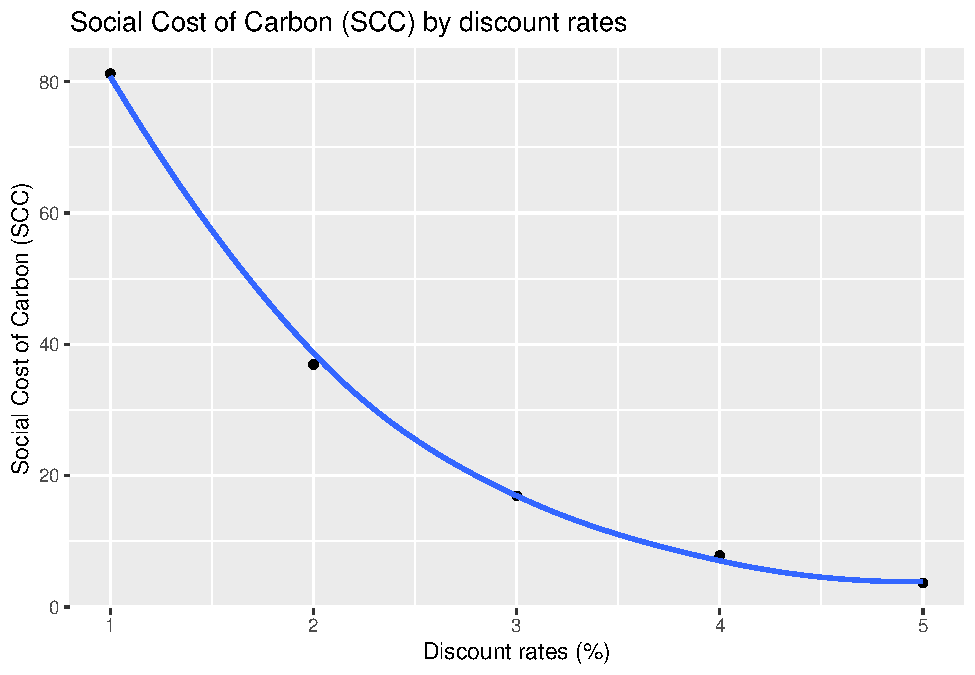
\includegraphics{Homework-4-Code_files/figure-latex/unnamed-chunk-5-1.pdf}

\hypertarget{question-4}{%
\subsubsection{Question 4}\label{question-4}}

\hypertarget{the-scc-with-a-discount-rate-of-2.1-is-34.15-calculated-using-the-ramsey-rule.-this-value-is-represented-on-the-plot-below-shown-in-coral.}{%
\paragraph{The SCC with a discount rate of 2.1\% is \$34.15 calculated
using the Ramsey Rule. This value is represented on the plot below,
shown in
coral.}\label{the-scc-with-a-discount-rate-of-2.1-is-34.15-calculated-using-the-ramsey-rule.-this-value-is-represented-on-the-plot-below-shown-in-coral.}}

\begin{Shaded}
\begin{Highlighting}[]
\CommentTok{\# Question 4 Ramsey Rule}
\NormalTok{p }\OtherTok{=}\NormalTok{ .}\DecValTok{001}
\NormalTok{n }\OtherTok{=} \DecValTok{2}
\NormalTok{g }\OtherTok{=} \FloatTok{0.01}

\NormalTok{r }\OtherTok{=}\NormalTok{ p }\SpecialCharTok{+}\NormalTok{ n}\SpecialCharTok{*}\NormalTok{g}

\NormalTok{r}
\end{Highlighting}
\end{Shaded}

\begin{verbatim}
## [1] 0.021
\end{verbatim}

\begin{Shaded}
\begin{Highlighting}[]
\NormalTok{SCC2}\FloatTok{.1} \OtherTok{=}\NormalTok{ ((}\FunctionTok{sum}\NormalTok{(warming\_scc}\SpecialCharTok{$}\NormalTok{damage\_annual\_cost))}\SpecialCharTok{/}\NormalTok{(}\DecValTok{1}\FloatTok{+0.021}\NormalTok{)}\SpecialCharTok{\^{}}\DecValTok{80}\NormalTok{)}
\NormalTok{SCC2}\FloatTok{.1}
\end{Highlighting}
\end{Shaded}

\begin{verbatim}
## [1] 34.14818
\end{verbatim}

\begin{Shaded}
\begin{Highlighting}[]
\CommentTok{\# Add 2.1\% discount rate SCC point on plot}
\FunctionTok{ggplot}\NormalTok{(}\AttributeTok{data =}\NormalTok{ discount\_scc, }\FunctionTok{aes}\NormalTok{(}\AttributeTok{x =}\NormalTok{ Discount\_rate, }\AttributeTok{y =}\NormalTok{ SCC)) }\SpecialCharTok{+}
  \FunctionTok{geom\_point}\NormalTok{() }\SpecialCharTok{+}
  \FunctionTok{geom\_smooth}\NormalTok{(}\AttributeTok{data =}\NormalTok{ discount\_scc, }\FunctionTok{aes}\NormalTok{(}\AttributeTok{x =}\NormalTok{ Discount\_rate, }\AttributeTok{y =}\NormalTok{ SCC), }\AttributeTok{span =} \DecValTok{1}\NormalTok{, }\AttributeTok{se =} \ConstantTok{FALSE}\NormalTok{) }\SpecialCharTok{+}
  \FunctionTok{labs}\NormalTok{(}\AttributeTok{title =} \StringTok{"Social Cost of Carbon (SCC) by discount rates"}\NormalTok{, }\AttributeTok{x =} \StringTok{"Discount rates (\%)"}\NormalTok{, }\AttributeTok{y =} \StringTok{"Social Cost of Carbon (SCC)"}\NormalTok{) }\SpecialCharTok{+}
  \FunctionTok{geom\_point}\NormalTok{(}\FunctionTok{aes}\NormalTok{(}\AttributeTok{x =} \FloatTok{2.1}\NormalTok{, }\AttributeTok{y =} \FloatTok{34.14818}\NormalTok{, }\AttributeTok{color =} \StringTok{"coral12"}\NormalTok{), }\AttributeTok{show.legend =} \ConstantTok{FALSE}\NormalTok{)}
\end{Highlighting}
\end{Shaded}

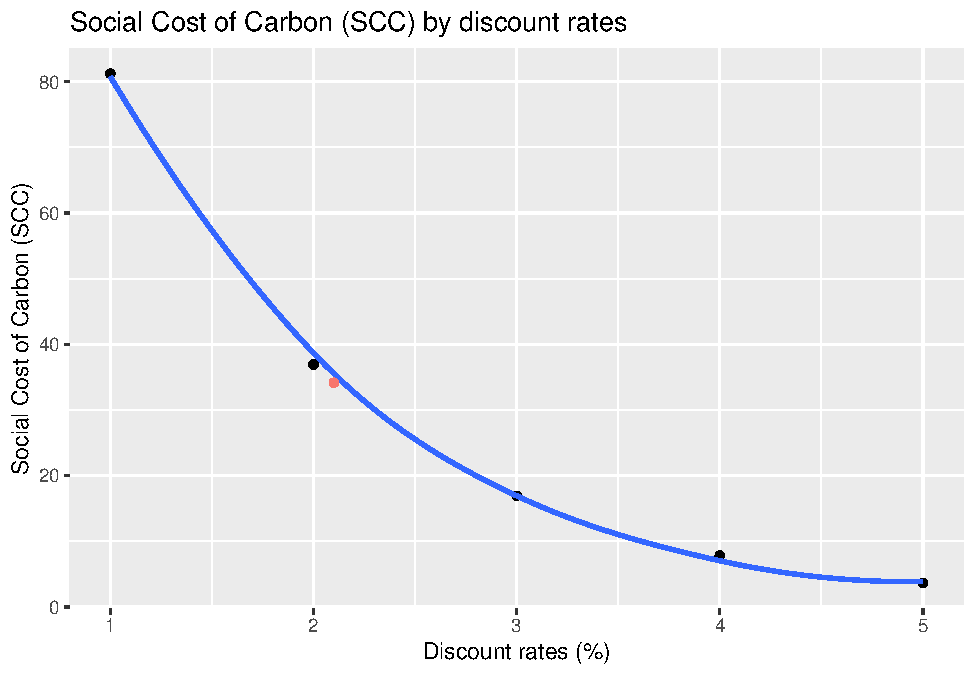
\includegraphics{Homework-4-Code_files/figure-latex/unnamed-chunk-6-1.pdf}

\hypertarget{question-5}{%
\subsubsection{Question 5}\label{question-5}}

\hypertarget{the-expected-present-value-of-damages-up-to-2100-under-policy-a-is-1869052186623438.}{%
\paragraph{The expected present value of damages up to 2100 under Policy
A is
\$1,869,052,186,623,438.}\label{the-expected-present-value-of-damages-up-to-2100-under-policy-a-is-1869052186623438.}}

\hypertarget{the-expected-present-value-of-damages-up-to-2100-under-policy-b-is-1422733591966428.}{%
\paragraph{The expected present value of damages up to 2100 under Policy
B is
\$1,422,733,591,966,428.}\label{the-expected-present-value-of-damages-up-to-2100-under-policy-b-is-1422733591966428.}}

\hypertarget{the-difference-between-damages-under-policy-a-and-policy-b-given-x-costs-for-policy-b-is-446318594657010.}{%
\paragraph{The difference between damages under Policy A and Policy B
given X costs for Policy B is
\$446,318,594,657,010.}\label{the-difference-between-damages-under-policy-a-and-policy-b-given-x-costs-for-policy-b-is-446318594657010.}}

\hypertarget{a-risk-averse-population-would-be-inclined-to-favor-policy-b-because-policy-a-has-a-50-probability-that-the-damages-will-be-greater-than-under-policy-b.-despite-policy-b-having-associated-costs-unlike-under-policy-a-it-still-is-more-economically-stable.}{%
\paragraph{A risk-averse population would be inclined to favor Policy B
because Policy A has a 50\% probability that the damages will be greater
than under Policy B. Despite Policy B having associated costs, unlike
under Policy A, it still is more economically
stable.}\label{a-risk-averse-population-would-be-inclined-to-favor-policy-b-because-policy-a-has-a-50-probability-that-the-damages-will-be-greater-than-under-policy-b.-despite-policy-b-having-associated-costs-unlike-under-policy-a-it-still-is-more-economically-stable.}}

\begin{Shaded}
\begin{Highlighting}[]
\CommentTok{\# Question 5}
\DocumentationTok{\#\# Expected present value of damages up to 2100 under Policy A }

\NormalTok{p1 }\OtherTok{=} \FloatTok{0.5}
\NormalTok{x\_1 }\OtherTok{=} \FunctionTok{sum}\NormalTok{(warming\_difference}\SpecialCharTok{$}\NormalTok{damage\_base)}\SpecialCharTok{/}\NormalTok{(}\DecValTok{1}\FloatTok{+0.02}\NormalTok{)}\SpecialCharTok{\^{}}\DecValTok{80}
\NormalTok{p2 }\OtherTok{=} \FloatTok{0.5}
\NormalTok{x\_2 }\OtherTok{=} \FunctionTok{sum}\NormalTok{(warming\_difference}\SpecialCharTok{$}\NormalTok{damage\_high)}\SpecialCharTok{/}\NormalTok{(}\DecValTok{1}\FloatTok{+0.02}\NormalTok{)}\SpecialCharTok{\^{}}\DecValTok{80}

\NormalTok{E }\OtherTok{=}\NormalTok{ (p1 }\SpecialCharTok{*}\NormalTok{ x\_1) }\SpecialCharTok{+}\NormalTok{ (p2 }\SpecialCharTok{*}\NormalTok{ x\_2)}

\NormalTok{E}
\end{Highlighting}
\end{Shaded}

\begin{verbatim}
## [1] 1.869052e+15
\end{verbatim}

\begin{Shaded}
\begin{Highlighting}[]
\DocumentationTok{\#\# Expected present value of damages up to 2100 under Policy B}
\NormalTok{policy\_b\_2050 }\OtherTok{\textless{}{-}}\NormalTok{ warming\_difference }\SpecialCharTok{\%\textgreater{}\%} 
  \FunctionTok{filter}\NormalTok{(year }\SpecialCharTok{\textless{}} \DecValTok{2051}\NormalTok{)}

\NormalTok{a }\OtherTok{=} \FunctionTok{sum}\NormalTok{(warming\_difference}\SpecialCharTok{$}\NormalTok{damage\_base)}
\NormalTok{b }\OtherTok{=}\NormalTok{ (}\FloatTok{2.853968e+13}\NormalTok{)}\SpecialCharTok{*}\DecValTok{50}
\NormalTok{a }\SpecialCharTok{+}\NormalTok{ b}
\end{Highlighting}
\end{Shaded}

\begin{verbatim}
## [1] 6.936451e+15
\end{verbatim}

\begin{Shaded}
\begin{Highlighting}[]
\NormalTok{E\_policy\_b }\OtherTok{=}\NormalTok{ (a }\SpecialCharTok{+}\NormalTok{ b)}\SpecialCharTok{/}\NormalTok{(}\DecValTok{1}\FloatTok{+0.02}\NormalTok{)}\SpecialCharTok{\^{}}\DecValTok{80}
\NormalTok{E\_policy\_b}
\end{Highlighting}
\end{Shaded}

\begin{verbatim}
## [1] 1.422734e+15
\end{verbatim}

\begin{Shaded}
\begin{Highlighting}[]
\DocumentationTok{\#\# Find the difference between damages under Policy A and Policy B given X costs for Policy B}
\NormalTok{X\_cost }\OtherTok{=}\NormalTok{ E }\SpecialCharTok{{-}}\NormalTok{ E\_policy\_b}
\NormalTok{X\_cost}
\end{Highlighting}
\end{Shaded}

\begin{verbatim}
## [1] 4.463186e+14
\end{verbatim}

\begin{Shaded}
\begin{Highlighting}[]
\DocumentationTok{\#\# A risk{-}averse population would be inclined to favor Policy B because Policy A has a 50\% probability that the damages will be greater than under Policy B. Despite Policy B having associated costs, unlike under Policy A, it still is more economically stable.}
\end{Highlighting}
\end{Shaded}


\end{document}
